\pgfplotsset{compat=1.3, 
small_thickness_axis/.style={
font=\sffamily,
every axis label/.append style={font=\sffamily}
}}

\begin{subfigure}[t]{0.48\textwidth}

\begin{tikzpicture}[]
\begin{groupplot}[
height=5cm,
width=0.65\linewidth,
group style={group size=2 by 1, horizontal sep=1em},
small_thickness_axis, xmode=log,
xticklabels={\10\textsuperscript{2}, 10\textsuperscript{3}, 10\textsuperscript{4}, 10\textsuperscript{5}, 10\textsuperscript{6}},
xmin=1e-7, xmax=1e-3,
ymax=2, 
legend style={
legend columns=2, column sep=5pt,
at={($(1,1)+(-1cm,0.3cm)$)}, anchor=south west, draw=none, font=\footnotesize\sffamily
},
]

\nextgroupplot[
xlabel={Thickness (nm)},
clip=false,
]
% This file was created by tikzplotlib v0.9.0.
\definecolor{color0}{rgb}{0.72156862745098,0.12156862745098,0.12156862745098}
\definecolor{color1}{rgb}{0.137254901960784,0.407843137254902,0.635294117647059}

\addplot [semithick, black, dashed]
table {%
6.30957344480193e-08 1
0.00158489319246111 1
};
\addplot [semithick, color0, mark=*, mark size=1, mark options={solid}, only marks]
table {%
1e-07 1.42993630573248
1.62377673918872e-07 1.40764331210191
2.63665089873036e-07 1.38216560509554
4.2813323987194e-07 1.35031847133758
6.9519279617756e-07 1.31847133757962
1.12883789168469e-06 1.28662420382166
1.83298071083244e-06 1.2515923566879
2.97635144163132e-06 1.21974522292994
4.83293023857175e-06 1.19108280254777
7.84759970351461e-06 1.16242038216561
1.27427498570313e-05 1.13694267515924
2.06913808111479e-05 1.11146496815287
3.35981828628378e-05 1.08917197452229
5.45559478116851e-05 1.07006369426752
8.85866790410083e-05 1.05414012738854
0.000143844988828766 1.04140127388535
0.000233572146909012 1.03184713375796
0.000379269019073225 1.02229299363057
0.000615848211066026 1.01592356687898
0.001 1.00955414012739
};
\addplot [semithick, color1, mark=square*, mark size=1, mark options={solid}, only marks]
table {%
1e-07 1.82520571949452
1.62377673918872e-07 1.50605361031323
2.63665089873036e-07 1.3207271200202
4.2813323987194e-07 1.21615276544283
6.9519279617756e-07 1.15799477120282
1.12883789168469e-06 1.11973166560983
1.83298071083244e-06 1.08681604296534
2.97635144163132e-06 1.06097619589036
4.83293023857175e-06 1.04270286157783
7.84759970351461e-06 1.03026414409083
1.27427498570313e-05 1.02504397690939
2.06913808111479e-05 1.02109676955645
3.35981828628378e-05 1.01847025853335
5.45559478116851e-05 1.01576562361788
8.85866790410083e-05 1.01296573032951
0.000143844988828766 1.01060474743796
0.000233572146909012 1.00918578064622
0.000379269019073225 1.00584658237861
0.000615848211066026 1.00403643474751
0.001 1.00099033181643
};

\legend{, $\displaystyle \frac{V_m}{V_m^{SQ}}$ , $\displaystyle \frac{J_m^{SQ}}{V_m}$ };
\node [anchor=north east] at (rel axis cs: 0.95, 0.95) {\ce{CuInSe2}};
\node [anchor=south west] at (rel axis cs: 0, 1.15) {\textbf{a}};
\node [anchor=south west] at (rel axis cs: 2.1, 1.15) {\textbf{b}};

\nextgroupplot[
xlabel={Thickness (nm)},
yticklabels={},
]
% This file was created by tikzplotlib v0.9.0.
\definecolor{color0}{rgb}{0.72156862745098,0.12156862745098,0.12156862745098}
\definecolor{color1}{rgb}{0.137254901960784,0.407843137254902,0.635294117647059}

\addplot [semithick, black, dashed]
table {%
6.30957344480193e-08 1
0.00158489319246111 1
};
\addplot [semithick, color0, mark=*, mark size=1, mark options={solid}, only marks]
table {%
1e-07 1.14654161781946
1.62377673918872e-07 1.13950762016413
2.63665089873036e-07 1.13012895662368
4.2813323987194e-07 1.11957796014068
6.9519279617756e-07 1.10785463071512
1.12883789168469e-06 1.09613130128957
1.83298071083244e-06 1.08440797186401
2.97635144163132e-06 1.07268464243845
4.83293023857175e-06 1.0609613130129
7.84759970351461e-06 1.05041031652989
1.27427498570313e-05 1.04103165298945
2.06913808111479e-05 1.031652989449
3.35981828628378e-05 1.02461899179367
5.45559478116851e-05 1.01875732708089
8.85866790410083e-05 1.01406799531067
0.000143844988828766 1.00937866354045
0.000233572146909012 1.00703399765533
0.000379269019073225 1.00468933177022
0.000615848211066026 1.00234466588511
0.001 1.00117233294256
};
\addplot [semithick, color1, mark=square*, mark size=1, mark options={solid}, only marks]
table {%
1e-07 2.4029631710625
1.62377673918872e-07 1.92622436033199
2.63665089873036e-07 1.63011071899831
4.2813323987194e-07 1.44695723164454
6.9519279617756e-07 1.32857360510645
1.12883789168469e-06 1.24714324158495
1.83298071083244e-06 1.18838354975699
2.97635144163132e-06 1.14526640683703
4.83293023857175e-06 1.11312385483929
7.84759970351461e-06 1.08900571307222
1.27427498570313e-05 1.06939145919721
2.06913808111479e-05 1.05125705627763
3.35981828628378e-05 1.03702453383025
5.45559478116851e-05 1.02610281792122
8.85866790410083e-05 1.01842889883047
0.000143844988828766 1.01208875093157
0.000233572146909012 1.00874117605575
0.000379269019073225 1.00571117377693
0.000615848211066026 1.00289611868334
0.001 1.001432869189
};

\node [anchor=north east] at (rel axis cs: 0.95, 0.95) {\ce{CuGaSe2}};

\end{groupplot}
\end{tikzpicture}

\end{subfigure}
~
\begin{subfigure}[t]{0.48\textwidth}

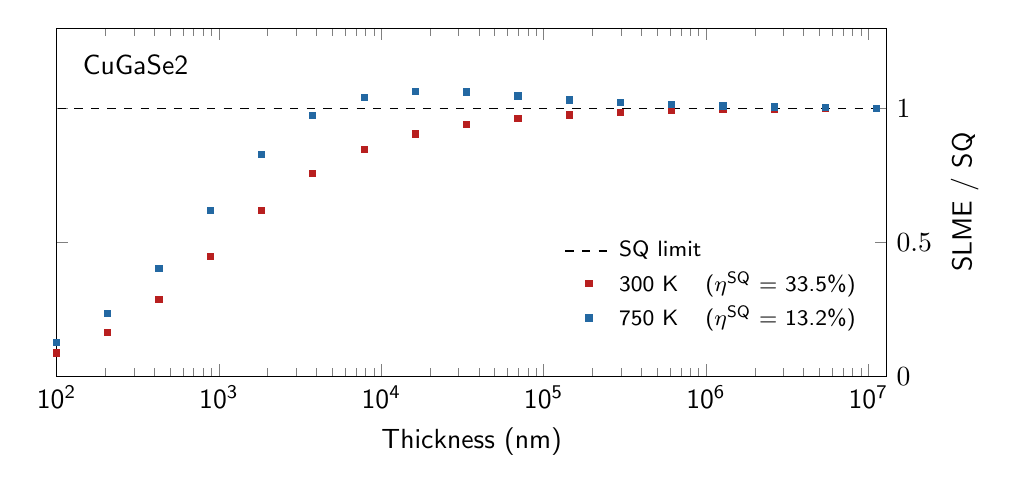
\begin{tikzpicture}[]
\begin{axis}[
width=\textwidth,
height=6cm,
small_thickness_axis, 
xlabel={Thickness (nm)}, xmode=log,
xticklabels={\textsf{10\textsuperscript{1}}, 10\textsuperscript{2}, 10\textsuperscript{3}, 10\textsuperscript{4}, 10\textsuperscript{5}, 10\textsuperscript{6}, 10\textsuperscript{7}},
xmin=1e-8, xmax=1.3e-3,
ymin=0, ymax=1.3,
ylabel={SLME / SQ},
yticklabel pos=right,
legend style={
at={(0.98, 0.1)}, anchor=south east, draw=none, font=\footnotesize\sffamily
},
legend cell align={left},
]

% This file was created by tikzplotlib v0.9.0.
\definecolor{color0}{rgb}{0.72156862745098,0.12156862745098,0.12156862745098}
\definecolor{color1}{rgb}{0.137254901960784,0.407843137254902,0.635294117647059}

\addplot [semithick, black, dashed]
table {%
5.01187233627269e-09 1
0.0199526231496887 1
};
\addlegendentry{SQ limit}
\addplot [semithick, color0, mark=square*, mark size=1, mark options={solid}, only marks]
table {%
1e-08 0.0866330601548305
2.06913808111479e-08 0.163427887334749
4.2813323987194e-08 0.285771424499606
8.85866790410083e-08 0.448102127054868
1.83298071083244e-07 0.618673919202687
3.79269019073225e-07 0.755717136961905
7.84759970351461e-07 0.846355206151773
1.62377673918872e-06 0.905057619927311
3.35981828628378e-06 0.941375809630965
6.95192796177561e-06 0.962027721833845
1.43844988828766e-05 0.975529139487879
2.97635144163131e-05 0.986516967951811
6.15848211066026e-05 0.993720951867257
0.000127427498570313 0.99700330024523
0.000263665089873036 0.998495602441319
0.000545559478116851 0.999352852930274
0.00112883789168469 0.999791387334807
0.00233572146909012 0.999958336723826
0.00483293023857175 1.0000178452293
0.01 1.00003013010135
};
\addlegendentry{300 K}
\addplot [semithick, color1, mark=square*, mark size=1, mark options={solid}, only marks]
table {%
1e-08 0.12452560452418
2.06913808111479e-08 0.233306944299895
4.2813323987194e-08 0.402877001561294
8.85866790410083e-08 0.618706879214286
1.83298071083244e-07 0.828471093287364
3.79269019073225e-07 0.972512729851043
7.84759970351461e-07 1.04116719118082
1.62377673918872e-06 1.06435411267563
3.35981828628378e-06 1.06203803311826
6.95192796177561e-06 1.04709930885196
1.43844988828766e-05 1.03164773271146
2.97635144163131e-05 1.02135936212352
6.15848211066026e-05 1.01456755607125
0.000127427498570313 1.0094574039516
0.000263665089873036 1.00564066148739
0.000545559478116851 1.00296488818489
0.00112883789168469 1.00136959899105
0.00233572146909012 1.00058694262244
0.00483293023857175 1.00028953487565
0.01 1.00021857093457
};
\addlegendentry{750 K}

\legend{SQ limit, 300~K \hspace{4pt} ($\mathsf{\eta^{SQ}}$ = 33.5\%) , 750~K \hspace{4pt} ($\mathsf{\eta^{SQ}}$ = 13.2\%)};
\node [anchor=north west] at (rel axis cs: 0.02, 0.95) {\ce{CuGaSe2}};
\end{axis}
\end{tikzpicture}

\end{subfigure}